\chapter{Описание заданного окружения}
\subsection{Общая схема сетевого взаимодействия сущностей}
В текущей работы рассматриваются три схемы и три СУБД расположенных удаленном сервере в отдельных \smallcode{Docker}-контейнерах:
\begin{itemize}
	\item База данных метаданных;
	\item База данных (margo?);
	\item База данных по игре Dota 2;
\end{itemize}

На \hyperref[fig:general-schema]{Рисунке \ref*{fig:general-schema}} представлена схема взаимодействия приложения управления метаданными и заданными базами данных.
\begin{figure}[h!]
	\centering
	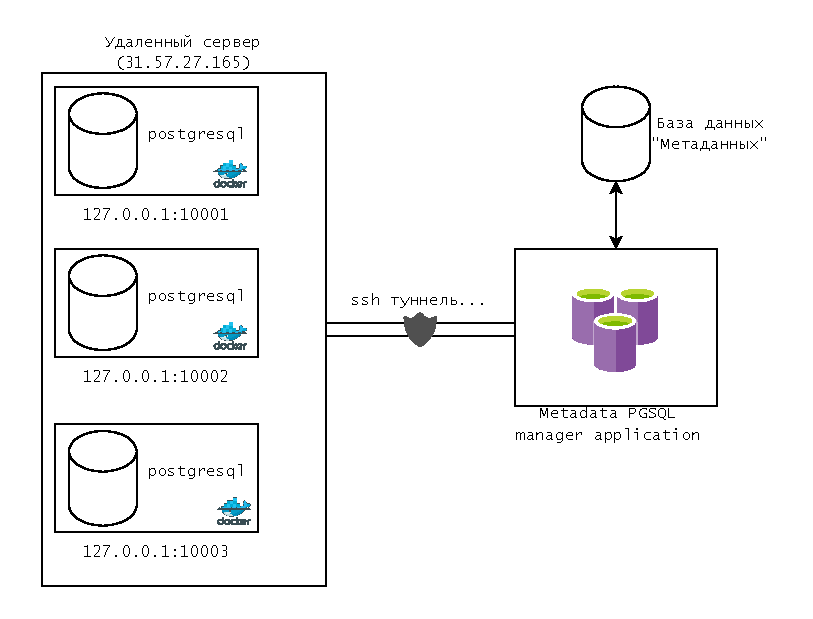
\includegraphics[width=1\linewidth]{docker-general-schema.drawio.pdf}
	\caption{Схема сетевого взаимодействия приложения и баз данных}
	\label{fig:general-schema}
\end{figure}

В рамках данной работы соединение с удаленным сервером с развернутыми СУБД выполнено через \texttt{SSH}-туннель.

\subsection{Развертывание и установка соединения с БД}
Для развертывания \texttt{Docker}-контейнеров были использованы \texttt{Docker-compose} скрипты представленные в \hyperref[lst:listing1]{Листинге \ref*{lst:listing1}}

\lstset{basicstyle=\ttfamily\small}
\begin{lstlisting}[language=bash, caption={docker-compose.yml файл для создания контейнера с СУБД	}, label={lst:listing1}]
services:
metadata-db:
	image: postgres:16
	container_name: metadata-db
	restart: unless-stopped
	env_file: .env
	ports:
		- "127.0.0.1:${VPS_PORT}:5432"
	volumes:
		- metadata_db_data:/var/lib/postgresql/data
volumes:
	metadata_db_data:
\end{lstlisting}

Параметр \texttt{VPS-PORT} задается в файле переменных окружения \texttt{.env}, пример файла представлен в  \hyperref[lst:listing2]{Листинге \ref*{lst:listing2}}

\begin{lstlisting}[language=bash, caption={.env файл для создания контейнера с СУБД}, label={lst:listing2}]
POSTGRES_DB=app
POSTGRES_USER=appuser
POSTGRES_PASSWORD=ChangeMe_12345
VPS_PORT=10001
\end{lstlisting}
В \texttt{.env} файле дополнительно настраиваются переменные окружения для подключения к базе данных: \texttt{POSTGRES\_DB}, \texttt{POSTGRES\_USER}, \texttt{POSTGRES\_PASSWORD}.

Для подключения к базе данных используется \texttt{DSN} (\texttt{Data soruce name}) по следующему шаблону:


\texttt{postgresql://[user[:password]@][host][:port]/[database\_name]}.

Для установки соединения необходимо настройку \texttt{SSH}-туннеля для портов, соответствующих контейнеров на удаленном сервере.

